\documentclass[12pt, a4paper]{report} \usepackage[titletoc]{appendix}
\usepackage{graphicx}
	\graphicspath{{images/}} 
\usepackage{geometry}
	\geometry{a4paper,left=3cm,top=3cm,bottom=3cm,right=3cm}
\usepackage{array}
\usepackage{multirow}
\usepackage{hyperref}
	\hypersetup{colorlinks=true,allcolors=blue}
\usepackage{hypcap}
\usepackage{csquotes}
\usepackage{subfig}

\setlength{\parindent}{1cm}
\setlength{\parskip}{0.1cm}

\usepackage{courier}
\usepackage{listings}
	\lstset{
  		basicstyle=\ttfamily\scriptsize,
  		frame=single,
  		breaklines=true,
  		numbers=left,
  		xleftmargin=2.5em,
  		framexleftmargin=0em,
  		emph={
        	class, extends, operation, abstract,
        	context, constraint, check,
        	for, if, return, true, and, ref,
        	message, in, package, val, attr, 
        	@link, @node, @compartment,
        	@namespace, @diagram
    	},
    	emphstyle=\textbf
	}
	\lstdefinestyle{interfaces}{
  		float=t!
	}


\begin{document}

\begin{titlepage}
 \begin{center}

\textbf{Progress Report}
\vspace{1cm}

\textbf{\large Model-Driven Gamified Software Modelling Learning}
\vspace{1cm}

Alfa Ryano Yohannis\\
ary506@york.ac.uk
\vspace{1cm}

Supervisors:\\
Dimitris Kolovos\\
Fiona Polack\\
\vspace{1cm}

Department of Computer Science\\
University of York\\
United Kingdom\\
\vspace{1cm}
\today
 
\vfill
 
\end{center}
\end{titlepage}


\begin{abstract}
\addcontentsline{toc}{chapter}{Abstract}
Motivated by the success of gameful approaches in different fields, this research harnesses the engaging nature of games combined with the effectiveness of pedagogy and the automation of Model-Driven Engineering to propose a framework for model-driven gamified software modelling learning. The framework allows tutors to create software modelling learning activities, and to generate software modelling learning games for learners to play. This report presents the motivation behind the framework and reviews the progress that has been made so far. A research plan is also presented to show remaining work that needs to be executed in the two and a half years.
\end{abstract}

\tableofcontents
\addcontentsline{toc}{chapter}{Contents}

\listoffigures
\newpage
 
\listoftables
\newpage

\lstlistoflistings
\newpage

\chapter{Introduction}
\label{Introduction}
In this section, the background, questions, objectives, potential outputs, and scoping of this research are presented.

\section{Background}
Software modelling is commonly perceived as a difficult subject since it
requires a mastery of abstraction \cite{Borstler2012}. However, this subject has a significant role in software engineering education and
practice. Successful application of software modelling requires skills in
abstract modelling \cite{whittle2013industrial}. The modelling itself is the process of thinking abstractly about system \cite{bezivin2009teaching}. Thus, teaching modelling also means teaching abstraction \cite{engels2005teaching}. Therefore, it is crucial to make students understand the value of abstraction \cite{bezivin2009teaching}. Weak software modelling skills will likely cause software engineering students to face further challenges with their degrees, as most of the software engineering related subjects involve of inherent abstraction problems \cite{Kramer2007}. Drawing from multidisciplinary research to define an abstraction for Artifical Intelligence, Saitta et al. stated that abstraction is often associated with these processes: information hiding, generalisation, approximation or reformulation, and separating relevant from irrelevant aspects \cite{Saitta2013}. Those processes are the common approaches applied in Computer Science, such as encapsulation and generalisation in object-oriented programming, resolution of polygon density in 3D modelling, algebraic simplification in symbolic computation, and removing colour information of images to produce grayscales. In the context of software engineering and computer science education, Kramer \cite{Kramer2007} and Hazzan \cite{hazzan2008reflections} argued that abstraction is the central theme or key skill for computing.

\begin{displayquote}
``I believe that abstraction is a key skill for computing. It is essential
during requirements engineering to elicit the critical aspects of the 
environment \dots At design time \dots Even at the implementation stage
\dots --- Kramer \cite{Kramer2007}.
\end{displayquote}

\begin{displayquote}
`` \dots software is an intangible object, and hence, requires highly developed
cognitive skills for coping with different levels of abstraction." --- Hazzan
\cite{hazzan2008reflections}.
\end{displayquote}

The problem of learning appropriate abstraction skills for software modelling is similar to problems in mathematics, where most of the concepts can only be accessed through symbolical representations \cite{Duval2006}. The abstract nature of software modelling traditionally has been addressed through the use of diagrams or visual notations in the form of modelling and diagramming tools. However, grasping concepts represented by the visual notations and conversely presenting back the concepts into visual notations are not trivial, including presenting aspects of the concept in different visual notation as well as choosing the right levels of abstraction and moving between them. Learning and teaching these skills are challenging. To overcome the challenges, a dedicated framework to support the learning of the modelling skills in a gamified way will bring significant benefits. 
 
The presence of learning framework does not guarantee will improve learners' engagement in software modelling learning. In recent years, the use of games and game elements, such as Gamification \cite{deterding2011game} and Serious Games \cite{Michael2005}, for purposes other than leisure has drawn significant attention. Gamified approaches have been proposed as solutions to motivational problems that emerge when users are required to engage in activities that they perceive as boring, irrelevant, or difficult. 

Real-world examples that show the success of the gamification are Duolingo\footnote{\url{https://www.duolingo.com/ }} and Re-mission\footnote{\url{http://www.re-mission.net/}}. Duolingo is a gamified system of language learning. It embeds game elements, such as points, levels,and lives, to make language learning more fun. Re-mission is a third-person shooting game dedicated to young cancer patients and designed to teach and learn how to deal with cancer. The patients are invited to take part in an entertaining gameplay that will affect their specific behavioural and psychological outcomes producing effective cancer therapy.
 
Through a systematic review, Connolly et al. \cite{connolly2012systematic} studied the impact of computer games and serious games on engagement and learning in diverse fields. They reported the majority of the studies presented empirical evidence about the positive impact of computer games and serious games. Using the same type of method, Hamari et al. \cite{hamari2014does} found that according to the majority of the reviewed papers, gamification does generate benefits and positive effects. Specifically in the field of software engineering, Pedreira et al. \cite{Pedreira2015} also performed a systematic review of the application of gamification in software engineering. Most existing studies focus on software development, project management, requirements, and other support areas, but none of them focuses on software modelling. They also found fewer studies reporting empirical evidence to support gamification research. They argued that existing research in the field are quite new. Thus more research effort is needed to investigate the impact of gamification in software engineering. Reports of the positive impact of gamification in various fields, particularly addressing engagement issues, encourage us to leverage it to deliver gamified software modelling learning, an area which has received little attention for the application of games and game elements so far. 

In terms of learning, pedagogical aspect cannot be neglected. Several concepts from pedagogy will be applied to drive the design of the framework, particularly the best practices from instructional design, a mature field in designing learning activities so that learning processes can be more efficient and effective. Therefore, incorporating gameful approaches as well as the best practices of instructional design will bring significant benefits to tackle the problems in learning software modelling. The framework is being designed to be suitable for higher-level undergraduate and postgraduate students with some experience of software engineering. 

Rather than just being a learning content for learners, software modelling also broadens opportunity to improve the meta-processes of the gamified software modelling learning, through the application of Model-Driven Engineering (MDE) approaches. Instead of developing the software modelling games manually, a model-based approach is applied. A framework is being developed, and it will act as a design framework to design learning activities for topics in software modelling. The learning activity design is then be transformed to generate gamified learning activities of software modelling. 

\section{Research Questions}
Thus, this research proposes the main research question ``What kind of framework that produces gamified learning activities to improve software modelling learning?". The word `framework' means a software environment for tutors and learners to design and perform gamified software modelling learning. The word 'produce' indicates the framework support tutors in designing and generating gamified learning activities. Thus, the framework should be expressive enough to support various visual modelling notations and the creation of different patterns of learning activities for learning software modelling. The word `improve' implies that learning with gameful approaches enhances learners' engagement and learning performance. They are more durable, frequent, and active compared to learners that only use didactic approach. Also, the former perform better in knowledge and skill acquisition and application compared to the latter. To answer the main research question, following sub research questions need to be investigated:
\begin{enumerate} 
\item Which game styles and elements are suitable for software modelling games?
\item Which of the aspects of developing a software modelling game can be automated through the use of model-driven engineering?
\item Do software modelling games improve learners' performance and engagement?
\end{enumerate}

\section{Research Objectives}
The solution proposed by this research is to produce a framework that can support tutors to design gamified learning activities as well as learners to learn software modelling in a gamified way. More precisely, this research aims to meet the following research objectives that are derived from the solution:
\begin{enumerate}
\item Investigate game styles and elements that are suitable for software modelling games, existing pedagogical approaches to optimise software modelling learning, and Model-Driven Engineering's best practices to automate software modelling game production.
\item Design and develop a framework that accommodates gamified and pedagogical approaches to be implemented through harnessing the best practices of Model-Driven Engineering. 
\item Perform controlled experiments to measure the significance of the framework in improving learning engagement and performance compared to traditional method---didactic learning without the support of gameful approaches.
\end{enumerate}

\section{Research Outputs}
By the end of this research, two possible research outputs have identified will have been produced:
\begin{enumerate}
\item A framework for tutors to design and produce gamified learning activities of software modelling and for learners to learn software modelling in gamified ways. 
\item Controlled experiments---comparison on learning engagement and performance of learners between gamified version and the traditional one of software modelling learning.
\end{enumerate}

\section{Research Scoping}
In the beginning, this research plans to address software modelling in Model-Driven Engineering as a whole---comprising modelling, metamodelling, and model transformation. However, after consideration regarding scope and time, it's scope is adjusted to focus on graphical software modelling, which is a common way to express models in modelling and metamodelling. Model transformation is excluded since its approaches are commonly expressed in a textual way, but still includes metamodelling as a metamodel itself is a model of models and usually is expressed in the form of class diagram-like graphics. This research plans to perform literature study and develop a prototype in the first and second years and address experiments for validation in the third year respectively.\newline\newline
The remainder of this report is organised as follows. A detailed
progress review is presented in Section \ref{Progres Review} and a research plan in Section \ref{Research Plan}. Section \ref{References} contains the references of this report and finally Section \ref{Publications} lists the publication of this research.

\chapter{Progress Review}
\label{Progres Review}
In this section, the progress of this research is reviewed. First, the Design Science Research Methodology (DSRM) \cite{peffers2007design}, the main research method employed in this research, is discussed briefly, and then followed by a discussion of progress on activities composing DSRM.

\begin{figure}[th] \centering 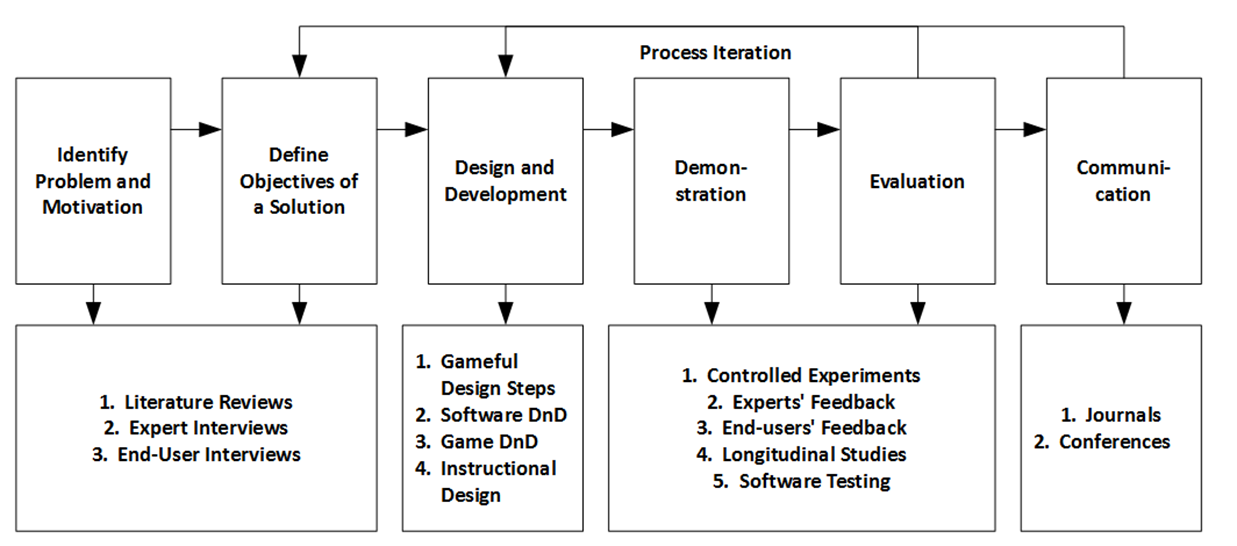
\includegraphics[width=\textwidth]{dsrm}
\caption{Design Science Research Methodology. Adapted from Peffer et al. \cite{peffers2007design}.}
\label{dsrm}
\end{figure}

\section{Research Methods}
\label{Research Methods}
Design Science Research Methodology (DSRM) is selected as the main research method since the main output of this research is a design artefact, a framework to design and generate gamified software modelling learning. DSRM provides a comprehensive conceptual framework and activity guidelines for understanding, developing, executing, and evaluating a design artefact (Figure \ref{dsrm}). Another reason is that it positions itself at the top level of abstraction without going into much detail of how to perform each activity, researchers can freely choose other more concrete research methods to carry out the activities. For examples, literature reviews, surveys, or expert interviews can be conducted to determine research problems, motivations, solutions, and objectives as well as controlled experiments to measure and evaluate the effectiveness of the artefacts. DSRM consists of six activities: identify problem and motivation, define objectives for a solution, design and development, demonstration and evaluation, and communication. The progress of this research on these six activities are discussed in the following sections.

\section{Identify Problems and Motivation}
Problem identification and motivation of this investigation have been widely presented in the Introduction section (Chapter \ref{Introduction}). In this section, they have restated again in a succinct manner. 

Software modelling plays a significant role in software engineering. However, its abstract nature makes it challenging to be mastered since most of its concepts are mostly presented in symbolical notations. To master software modelling, learners need to possess modelling skills, such as grasping ideas behind models presented in visual modelling notations, presenting back the ideas into visual modelling notations, viewing the ideas from different perspectives using different visual modelling notations, choosing the right levels of abstraction of modelling and moving between. Acquiring these skills might be difficult enough to demotivate learners from learning software modelling.

Apart from the problems previously mentioned, the use of games or game elements rises as solutions to tackle motivational problems. Also, pedagogy has been a mature field to deliver effective learning processes. Therefore, incorporating gameful approaches as well as the pedagogy's best practices can bring significant benefits to tackle the problems in learning software modelling. A framework that unifies the gameful and pedagogical approaches are needed. This is where Model-Driven Engineering plays it role. Not just being content in software modelling learning, Model-Driven Engineering provides best practices to automate, customise, and reuse gamified learning activities. Thus, this research is motivated to produce a framework that can support tutors to design gamified learning activities and learners to learn software modelling gamefully.


\section{Define Objective for a Solution}
The objective for a solution proposed by this research is to develop a framework that can support tutors to design gamified learning activities as well as learners to learn software modelling in a gamified way. 

The design of a solution should be rigorously defined to ensure the solution to work. It means the design should be based on existing foundations (models, theories, frameworks, etc.) \cite{von2004design}. Thus, some requirements have to be met to ensure the framework has appropriate quality. Some requirements have been identified---pedagogical requirements and gaming requirements---and they are gathered from two sources, from the literature review and a preliminary survey. These requirements have two roles. First, they provide guidance to design process and, second, they will also act as units of evaluation to confirm the framework meets certain qualities and functionalities.

\subsection{Pedagogical Requirements}
\label{Pedagogical Requirements}
Pedagogical requirements are classified into three categories, requirements from pedagogy-psychology literature, requirements from software modelling learning' best practices, and requirements from a preliminary survey. They are presented in the following subsections.  

\subsubsection{Requirements from Pedagogy-Psychology Literature}
\label{Requirements from Pedagogy-Psychology Literature}
Bloom's taxonomy is a model that categorise learning activities into six levels based on their cognitive load incrementally; the six levels are remember, understand, apply, analyse, evaluate, and create \cite{krathwohl2002revision}. Performing activities in \emph{create} category is more challenging than activities in the lower categories since they demand high cognitive loads. All of these activities, whether they are arranged gradually or a combination of them, can give different variation and difficulty of a challenge to learners when they are performed in a learning context. 

While learners are progressing in the framework, they are developing their competence. Thus, difficulty has to be kept balanced with their competence. Otherwise, they will get bored. It is the situation where the Flow concept \cite{csikszentmihalyi2014toward} can be applied. There are three have been identified so far related to a pedagogical approach to control the degree of difficulty: a combination of Bloom's activities, the introduction of new concepts, and application in different domains. The order of the levels of each of the three ways has to be arranged properly following the Flow theory. Concepts that are easier are given earlier than the harder ones, and the difficulty is gradually increased as learners progress. Likewise, Application in the domains that are more familiar with learners should be given first and gradually shifted to the domains that are most unfamiliar. Combining these three dimensions--types of activities, concepts, and domains--could provide us with a variety of levels with different degrees of difficulties. 

Motivation is an important aspect in the success of learning, and Keller's ARCS motivational model is also selected to address this aspect \cite{keller2010motivational}. The model provides us in each its components---attention, relevance, confidence, satisfaction---a set of predefined techniques to maintain learners' motivation. In the course of a level of the framework, there are a start, an end, and learning activities in between. The ARCS' techniques can be applied to maintain learners' motivation along the course of completing a level. As an example, the animation could be used to gain learners' attention, explaining the application of the concept being taught in the currently playing level to give relevance, showing their progress in completing a level to maintain their confidence and giving them a reward after finishing a level for reward. 
 
The concept of Scaffolding \cite{vygotsky1978mind, wood1976role} could also be applied to support learners coping challenges. Throughout finishing a level, scaffolding could be provided in several ways: reducing extensive modelling activities into smaller activity constituents, removing irrelevant activities, providing an almost complete model so they can work on the most relevant activities rather than build the model from scratch, provide help and documentation, and give some clues of the solutions when they get stuck. This support will be reduced as players progress to maintain the balance between their increasing competence and difficulty. Scaffolding is not generated automatically by the framework. Instead, tutors are given freedom to incorporate scaffolding into their learning activity design. 

Kolb's experiential learning model \cite{kolb2014experiential} is also applied to the framework. The model agrees knowledge is constructed through experience and based its model on constructivism \cite{kolb2014experiential}. Kolb's model was selected since playing levels in the framework is similar to the learning cycle Kolb proposed. The cycle consists of 4 steps: concrete experience, reflective observation , abstract conceptualisation, and active experimentation. 

So far, different concepts in pedagogy and psychology related to learning have been identified---from Bloom's taxonomy to Kolb's experiential learning---and of course, there many other related existing concepts that have not been investigated. All of these concepts are believed can provide principles that are useful to deliver an effective learning. Thus, instead of rigorously design the framework only to certain concepts, it's better to allow tutors to apply these different concepts of learning into their learning activity design. Thus, this research aims to make the framework generic enough to accommodate different learning approaches. However, as a start, some concepts still have to be selected to guide and validate the design of the framework. Thus, the concepts presented in this subsection are also chosen as the requirements for the design of the framework (Table \ref{design-learning-models}).

\begin{table}[t!]
\caption{Requirements derived from learning theories and models.}
\label{design-learning-models}
\begin{center}
\begin{tabular}{ p{2.3cm}p{1cm}p{9.7cm} } 
\hline
Category & Code & Requirements from Pedagogy-Psychology Literature\\
\hline
\multirow{1}{2cm}{Pedagogical-Psychological Concepts} 
& RM01 & The framework facilitates the Bloom's taxonomy \cite{krathwohl2002revision}. \\
& RM02 & The framework accomodates Kolb's experiential learning model \cite{kolb2014experiential}. \\ 
& RM03 & The framework allows Keller's ARCS motivational model \cite{keller2010motivational}. \\
& RM04 & The framework enables scaffolded learning \cite{vygotsky1978mind, wood1976role}. \\
& RM05 & The framework supports the theory of Flow \cite{csikszentmihalyi2014toward}. \\ 
\hline
\end{tabular}
\end{center}
\end{table}

\subsubsection{Requirements from Software Modelling Learning}
\label{Requirements from Software Modelling Learning}
Requirements from software modelling learning are the best practices pointed out by experts in the field about what and how software modelling should be taught and learnt. These requirements are used as key points to consider in the design phase of the gamified software modelling learning framework. The list of the identified requirements can be seen in Table \ref{literature-review-1}. 

Since contents, practices, and tools design in the list are vary and recommended from different experts, it is more generic if the framework can allow tutors to express these best practices into their learning activities based on their own preferences and needs rather than fixedly embed all the requirements into the framework. The word 'generic' means the learning activities can be reused and modified based on their contextual use.

\begin{table}[t!]\caption{Requirements derived from the literature review.}
\label{literature-review-1}
\begin{center}
\begin{tabular}{ p{1.6cm}p{1cm}p{10.4cm} } 
\hline
Category & Code & Framework's Requirements from Literature Review \\
\hline
\multirow{1}{2cm}{Contents} 
& RL01 & Teach MDE Definition \cite{borstler2012teaching}. \\ 
& RL02 & Teach semantics, syntaxes, notations \cite{borstler2012teaching}. \\ 
& RL03 & Teach Modelling, metamodelling, model validation, model transformation \cite{bezivin2009teaching, ober2007teaching}. \\
& RL04 & Teach the applications of MDE \cite{bezivin2009teaching, liebel2015ready}. \\
& RL05 & Teach the engineering aspect of modelling \cite{paige2014bad}.\\
& RL06 & Teach modelling in various domains and contexts \cite{borstler2012teaching, paige2014bad}.\\
\hline
\multirow{1}{2cm}{Practices} 
& RL07 & Teach that modelling is abstract thinking \cite{bezivin2009teaching}.\\
& RL08 & Learners should at least are proficient in object-orientation \cite{bezivin2009teaching, paige2014bad, Akayama2013}.\\
& RL09 & Measure student's model's quality \cite{Akayama2013}.\\
& RL10 & Facilitate teaching problem solving first, detail specifications and tools get in the way \cite{paige2014bad}. \\
& RL11 & Provide support to solutions, not direct answers \cite{paige2014bad}. \\ 
& RL12 & Facilitate teaching broadly, throughout, not deeply \cite{borstler2012teaching, paige2014bad, Akayama2013}.\\
& RL13 & Facilitate teaching with different modelling languages \cite{bezivin2009teaching, paige2014bad}.\\ 
& RL14 & It is engaging (fun, challenging) \cite{paige2014bad}.\\ 
& RL15 & Teach from ground, real-world, familiar objects, up to abstraction \cite{engels2005teaching}.\\ 

\hline
\multirow{1}{2cm}{Tool Design}
& RL16 & Have adequate support and documentation \cite{liebel2015ready}. \\
& RL17 & Designed to build knowledge incrementally \cite{lethbridge2014teaching}.\\
& RL18 & Provide flexibility to explore learning \cite{lethbridge2014teaching}. \\
& RL19 & Give positive reinforcement \cite{lethbridge2014teaching}. \\
& RL20 & Convince the value of the topic being learned \cite{lethbridge2014teaching}. \\ 
& RL21 & Have high usability \cite{lethbridge2014teaching}.\\ 
\hline
\end{tabular}
\end{center}
\end{table}

\subsubsection{Requirements from A Preliminary Survey}
\label{Requirements from A Preliminary Survey}
A preliminary survey to identify learners' needs, motivations and challenges have been conducted according to the Research phase of the Deterding's Gameful Design Framework \cite{deterding2015lens}. The preliminary survey aims to identify the requirements in designing the gameful aspect of the framework. It is not intended to measure significance, but it is a qualitative investigation to reveal needs, motivations, and challenges in learning software modelling from learners' perspective. The preliminary survey is also in line with the Design Science Research Methodology \cite{peffers2007design}, in order to identify the problem and motivation so that this research can define the objective of a solution accurately in the second activity.

Online questionnaires were distributed to students of Model Driven Engineering (MODE) 2015/2016 module. The students were in their Software Engineering master programme at the University of York. From 21 students, only 4 completed the questionnaires. Since the number of respondents are small for generalisation, the same survey is planned to applied to next term MODE students, and the result is only used to confirm and backup requirements from software modelling learning' best practices (Section ) and requirements from pedagogy-psychology literature.

From the requirement identification, it is found that the requirements derived from the preliminary survey (Table \ref{preliminary-survey}) support and confirm the requirements from pedagogy-psychology literature (Table \ref{design-learning-models}) and from software modelling learning literature (Table \ref{literature-review-1}). 

\begin{table}[t!]
\caption{Requirements derived from the preliminary survey.}
\label{preliminary-survey}
\begin{center}
\begin{tabular}{ p{2cm}p{1cm}p{10cm} } 
\hline
Category & Code & Requirements from Preliminary Survey \\
\hline
\multirow{1}{2cm}{Needs} 
& RS01 & Teach them knowledge and skills that are applicable in industry: model management (abstract thinking, modelling, metamodelling, model transformation, validation, and application) and tool literacy. \\ 
\hline
\multirow{1}{2cm}{Motivations}
& RS02 & Promote gaining advance knowledge and skills in MDE. \\ 
& RS03 & Promote the benefits and applications of MDE. \\ 
\hline
\multirow{1}{2cm}{Interesting Challenges}
& RS04 & Challenge with model management activities (abstract thinking, model validation, metamodelling, etc.). \\ 
& RS05 & Scaffold learning process to support learners gaining their experience (for an example, dividing the activities into smaller activity chunks). \\ 
\hline
\multirow{1}{2cm}{Un-interesting Challenges}
& RS06 & Increase the usability of the tool being used. \\ 
& RS07 & No need to learn the detailed technical terms specific to certain products. \\ 
& RS08 & Provide documentation and support for the tools being used. \\ 
\hline
\end{tabular}
\end{center}
\end{table}


\subsection{Gaming Requirements}
\label{Gaming Requirements}
The main challenge addressed in this work is transforming software modelling learning into gameful activities. Given that there are different types of modelling languages (e.g. graphical, textual, projectional, tree-based) and types of games (continuous vs. level-based, real-time vs. turn-based, single-player vs. multi-player), at this stage it is worth noting that our study is limited to level-based single-player games for languages with a 2D graphical syntax. For this style of game, the following concerns and challenges have been identified. These concerns and challenges are summarised as requirements and listed in Table \ref{gaming-requirements}.

\subsubsection{Game Mechanics} 
\label{Game Mechanics} 
Gameful design method \cite{deterding2015lens} suggests that to apply gamification, the core activity should be identified before gameful modification can be implemented. Modelling using graphical modelling languages, such as constructing and modifying diagrams, mainly involves design, editing, and planning activities. The LM-GM framework \cite{arnab2015mapping} mentions these activities as game mechanics that can be used for learning, specifically to address the \emph{creating} category in Bloom's taxonomy \cite{krathwohl2002revision}. Thus, the activity of constructing and modifying diagrams can be used as game mechanics as well, as it also involves design, editing, and planning activities as in design, editing, and planning game mechanics.

As for gameplay, learners are asked to construct or modify diagrams so that the diagrams become consistent with a given problem description and instruction. They do not always have to start with an empty canvas but could start from existing, incomplete diagrams that are pre-made to help them focus on the core concepts and activities being taught \cite{deterding2015lens}. We name this kind of play as `construction gameplay'. Other forms of play can be supported. For example, learners can be provided with a problem description and a number of diagrams reflecting candidate solutions and asked to select the correct solution(s). In another form, learners can be given a diagram and a number of statements in natural language and choose the proper interpretation(s) or statement(s). We call these two forms of play `multiple-choice gameplay'. Tutors need to be able to define multiple levels of different gameplays and link them up to assemble complex games. 

For construction gameplay, a graphical editor through which the user can construct/modify solutions is needed. Ideally, the editor should be fully integrated into the game to provide live feedback and an immersive experience. An alternative is to ask the user to create/edit models in an existing modelling tool and upload them to the game. To simplify the definition of graphical editors embedded in the game, a standardised way to define the abstract and graphical syntaxes of supported languages is required. 

\subsubsection{Assessing Correctness} 
\label{Assessing Correctness} 
There are several ways to assess consistency and correctness for the construction gameplay. One option is to require that the provided diagram is a 1:1 match with a reference solution given by the game designer. A more relaxed approach is only to require that the provided solution satisfies a number of constraints. Another option is to require some form of semantic equivalence between the two models (e.g. class diagrams that are consistent with an object diagram). 

\subsubsection{Rewards}
\label{Rewards}
Rewards are a major element of learning games, allowing users to develop a sense of achievement, show off their new skills, and compare themselves against other users, etc. So far, two types of rewards have been selected, positive reinforcement and achievements. Positive reinforcement can have the form of sounds, visual effects, or motivating messages to give feedback to players. Positive reinforcement is intended to improve the self-efficacy of players by letting them know whether their actions are in the right direction, so they can decide and continue to execute their next actions \cite{richter2015studying}. Another reward is a list of a learner's achievements, which can act like a `CV' for a learner. It records the names, types, and numbers of levels and learning activities that they have been completed. Since a learning activity usually addresses a concept in software modelling, this could be used as a base to claim that the learners have acquired the competence -- knowledge and skill -- for that concept \cite{richter2015studying}. Building a learner's competence also means strengthening their intrinsic motivation \cite{ryan2017self} and make game playing  activities important to them \cite{nicholson2015recipe}.

\begin{table}[t!]
\caption{Gaming Requirements.}
\label{gaming-requirements}
\begin{center}
\begin{tabular}{ p{2cm}p{1cm}p{10cm} } 
\hline
Category & Code & Gaming Requirements\\
\hline
\multirow{1}{2cm}{Game Mechanics}
& GM01 & construction gameplay \cite{arnab2015mapping}\\
& GM02 & multiple-choice gameplay (selecting the best diagram)\\
& GM03 & multiple-choice gameplay (select the best interpretation)\\
\hline
\multirow{1}{2cm}{Assessing Correctness}
& GC01 & complete match validation\\
& GC02 & partial match validation\\
& GC03 & semantic equivalence validation\\
\hline
\multirow{1}{2cm}{Rewards}
& GR01 & positive reinforcement \cite{richter2015studying}\\
& GR02 & list of achievements \cite{richter2015studying}\\
\hline
\end{tabular}
\end{center}
\end{table}

\section{Design and Development}
A web-based prototype of the framework has been developed to facilitate the design and implementation of software modelling games in line with the concerns discussed in the Pedagogical Requirements (Section \ref{Pedagogical Requirements}) nad Gaming Requirements (Section \ref{Gaming Requirements}). The prototype implements a metamodel-annotation-based approach for defining the concrete syntax of the targeted modelling languages. Metamodels are defined in Ecore \cite{steinberg2008emf} and their concrete syntax is specified using Eugenia-like annotations\footnote{\url{http://www.eclipse.org/epsilon/doc/articles/eugenia-gmf-tutorial/}} \cite{kolovos2015eugenia}. Tutors can define a class as the root object of a metamodel (annotated with {\fontfamily{pcr}\selectfont @diagram}), denote classes to appears as nodes ({\fontfamily{pcr}\selectfont @node}) or links ({\fontfamily{pcr}\selectfont @link}), and denote a containment references to appear as compartments where elements of the type of the reference can be nested/spatially contained ({\fontfamily{pcr}\selectfont @compartment}). The instances of the annotated classes are displayed as visual elements in a web-based graphical editor built upon the MxGraph framework\footnote{\url{https://jgraph.github.io/mxgraph/}}. Tutors can adjust the appearance of the visual elements by setting the values of appropriate annotation parameters (for example, see Listing \ref{metamodel} and Figure \ref{example-01}-\ref{example-03} for the visual elements produced).

\begin{figure}[t!]
\centering
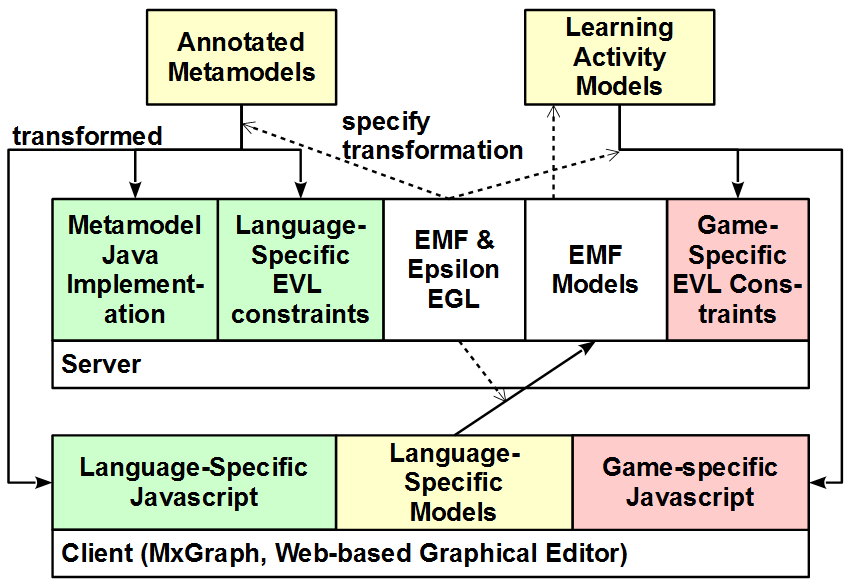
\includegraphics[width=12cm]{artefacts}
\caption{The framework's artefacts of the gamified software modelling learning.}
\label{artefacts}
\end{figure}


An annotated metamodel is then transformed using Epsilon EGL \cite{kolovos2010epsilon} and EMF \cite{steinberg2008emf} to generate its Java implementation code for further model management operations on the server, such as model validation and transformation (Figure \ref{artefacts}). The transformation also produces Javascript that implements a language-specific web-based graphical editor built on top of the MxGraph framework. After the generation, tutors can create language-specific models using this editor and validate them using language-specific EVL \cite{kolovos2006eclipse} constraints (Figure \ref{artefacts}). The models (the EMF models in Figure \ref{artefacts}) can be used as base models in construction gameplay and are required as candidate solutions, and as diagrams to be selected and interpreted by learners in multiple-choice gameplay.  

A modelling language has also been defined to design and link up different types of levels (see Figure \ref{laml} for its metamodel). We name the models constructed by this modelling language, \emph{learning activity models} (for example, see Figure \ref{eoml}). Currently, elements that are supported by the learning activity modelling language are activity, objective, model, start, end, transition, and link. The activity element represents an activity in a learning process (in the transformation that follows each activity is transformed to a level). In an activity, tutors need to define \emph{lesson} (description of the topic being taught), \emph{instruction} (direction to complete the activity), the name of the target metamodel, and a set of \emph{objectives}(elements to describe targets/conditions that learners have to meet in order to complete an activity). 

A \emph{model} is an element that refers to an existing model (the EMF models in Figure \ref{artefacts}) created by tutors or a target model that will be produced by an activity. The referred model is used as the base model when learners start an activity, so they don't have to create the referred model from scratch. The \emph{start} and \emph{end} elements indicate where a learning activity should start and end. A \emph{transition} element is a directed edge that connects one activity to another, and \emph{link} element is also a directed edge that connects a model to an activity and \textit{vice versa}. Facilitating tutors to create different learning activity models as well as to construct different models as base models for various visual modelling languages allows tutors t1o adjust the difficulty and support provided. This facility enables tutors to create various learning contents and activities that accommodates different learning approaches. Thus, it addresses some requirements in Subsection \ref{Pedagogical Requirements}.

Learning activity models are consumed by a model-to-text transformation to generate game-specific Javascript that implements a complete playable game (Figure \ref{artefacts}). The framework can host a number of generated games and provides features such as authentication, progress management, learning activity inventory, model inventory, etc.  

The generation also produces a game-specific EVL skeleton (Figure \ref{artefacts}) for each level where tutors can define constraints and operations used for validation, to determine whether the level has been completed and all its objectives have been met. Currently, only the construction gameplay is supported at each level, and the correctness of solutions is assessed using the EVL constraints. So far with EVL, tutors can create rules to perform 1:1 match validation between a diagram and a reference solution and to check that a solution satisfies a number of constraints (assessing correctness requirement in Subsection \ref{Assessing Correctness} is addressed). The multiple-choice gameplay (Subsection \ref{Game Mechanics}), and other validation approaches (Subsection \ref{Assessing Correctness}), as well as reward mechanisms (Subsection \ref{Rewards}), are in development. 


\section{Demonstration and Evaluation}

\subsection{Demonstration}
In this section, an example is presented to demonstrate the use of the framework in a game that introduces the concept of substates in UML statechart modelling. Learners are assumed to already understand the concepts of state, transition, start state, and final state. The following subsections present the different stages of the lifecycle of the game from definition to full use in game play.

\begin{figure}[t!]
\centering
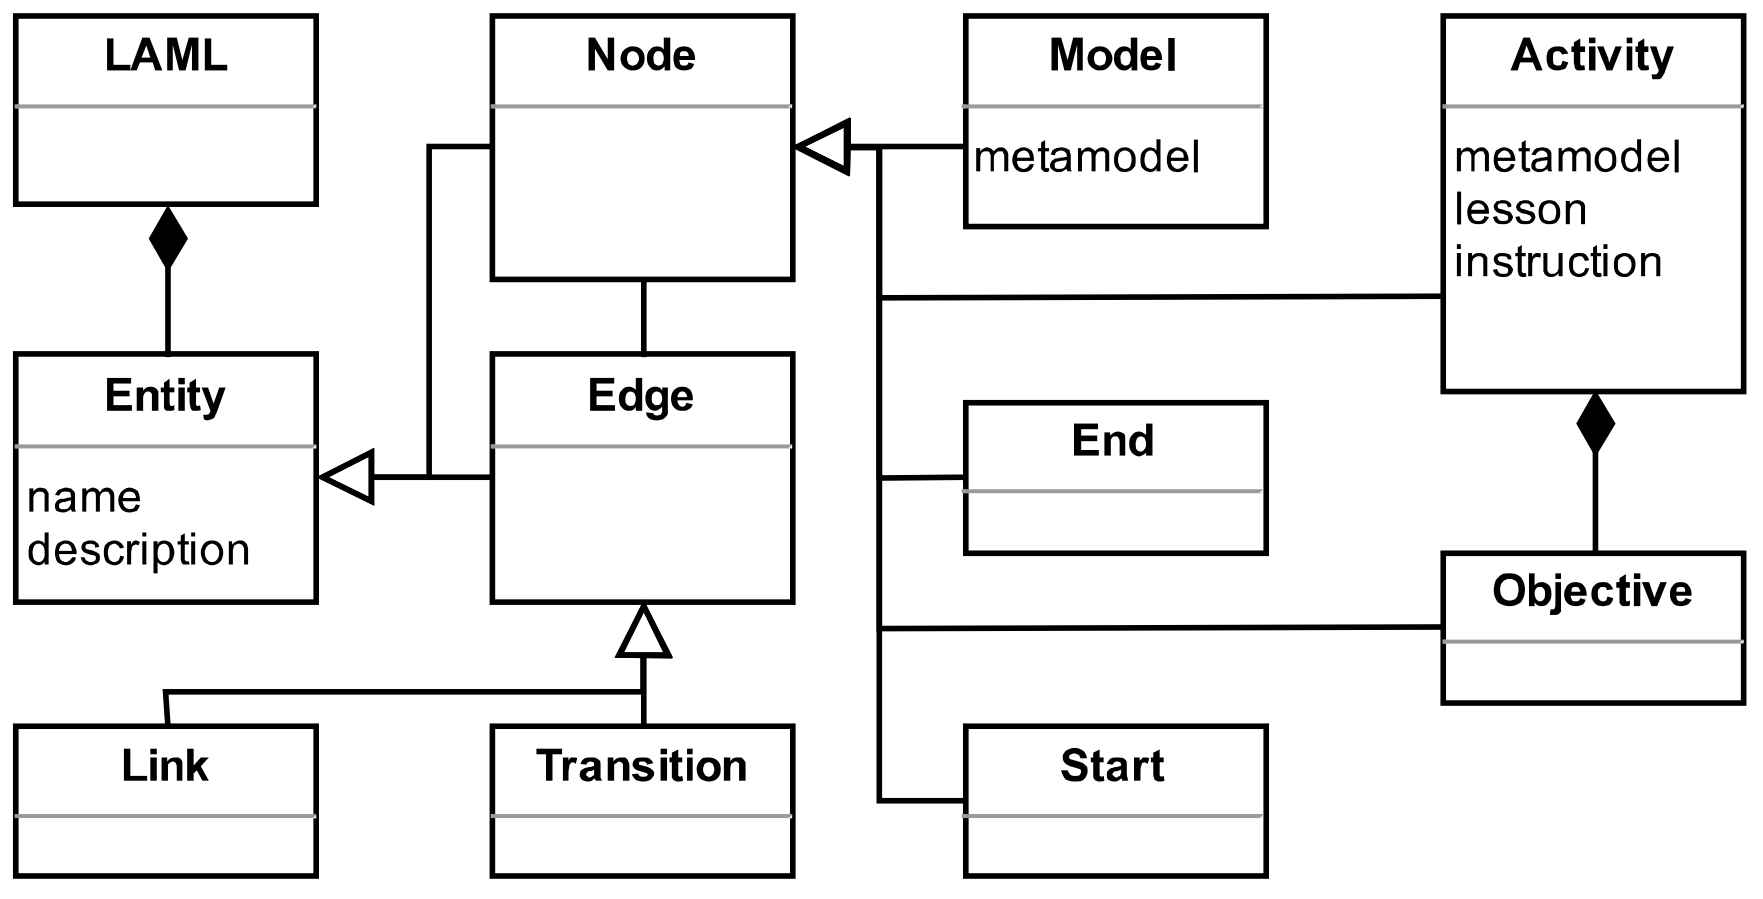
\includegraphics[width=12cm]{laml}
\caption{The class diagram of the \emph{learning activity modelling language}.}
\label{laml}
\end{figure}

\begin{lstlisting}[style=interfaces,caption={A definition of statechart diagram using Emfatic and Eugenia-like annotations.},label=metamodel]
@namespace(uri="statechart", prefix="statechart")
package statechart;

@diagram
class Statechart {
  val Entity[*] entities;
}
abstract class Entity {
  attr String name = "";
  attr String description = "";
}
abstract class Node extends Entity {
  ref Edge[*]#source outgoing;
  ref Edge[*]#target incoming;
}
abstract class Edge extends Entity {
  ref Node#outgoing source;
  ref Node#incoming target;
}
@link(label="name", source="source", target="target", label="name", endArrow="block", blockendFill="1", endSize="6", width="120", height="120")
class Transition extends Edge {
}
@link(label="name", source="source", target="target", label="name", endArrow="none", blockendFill="1", endSize="6", width="120", height="120", dashed="1")
class Link extends Edge {
}
@node(label="name", shape="swimlane", childLayout= "stackLayout", collapsible="1", horizontalStack="0", resizeParent="0", resizeLast="1", rounded="1", marginBottom="7", marginLeft="7", marginRight="7", marginTop="7", whiteSpace="wrap", width="200", height="120", swimlaneFillColor="#FFFFFF")
class State extends Node {
  @compartment(shape="swimlane", collapsible= "0", noLabel="1", editable="0", strokeColor="none", startSize="0")
  val State[*] substates;
}
@node(label="description", shape="note", whiteSpace="wrap", width="200", height="120")
class Note extends Node {
}
@node(label="name", shape="startState", whiteSpace="wrap", fillColor="#000000", width="30", height="30")
class Start extends Node {
}
@node(label="name", shape="endState", whiteSpace="wrap", fillColor="#FFFFFF", width="30", height="30")
class End extends Node {
}
\end{lstlisting} 

\subsubsection{Define Statechart Metamodel}
For the framework to support statechart modelling, designers need to define an annotated statechart metamodel as shown in Listing \ref{metamodel}. In line 1 and 2, the namespace and package of the metamodel are defined by setting uri, prefix, and package to ``statechart". Next, Statechart class is defined and annotated with {\fontfamily{pcr}\selectfont @diagram} to denote that the object of the Statechart class is the root object of the metamodel (the diagram). This class has a containment reference named `entities' with of type Entity. Thus, all instances of Entity and its subclasses can be contained in a Statechart diagram (lines 4-7).  

The statechart diagram is intended to only support six basic elements: state, note, start, end, transition and link. Therefore, six classes are specified to represent the elements (lines 21, 24, 27, 32, 35, 38). State, note, start, and end elements are nodes in the diagram; their classes are derived from Node class, and each is annotated with {\fontfamily{pcr}\selectfont @node}, as well as its MxGraph-related attributes (fillColor, width, height, shape, etc.), to determine its appearance in the diagram (lines 26, 31, 34, 37). Similarly, transition and link are edges in the diagram, extend the Edge class and are annotated with {\fontfamily{pcr}\selectfont @link} (lines 20, 21, 23, 24). The State class has a containment reference named substates that also has type State class. This means that an instance of State class can also contain other instances of State class as its substates. The \emph{substates} attribute is annotated with {\fontfamily{pcr}\selectfont @compartment} which means, in the diagram, a state has a container and other states can be placed inside it to become its substates (lines 28-29). The Node class has two references: outgoing and incoming. Both have the same type, Edge (lines 13-14). The Edge class also has two references: source and target. Both have the same type, Node class (lines 17-18).



\subsubsection{Create Statechart Model}
Using the generated graphical editor (Figure \ref{ide}), designers can now create statechart models. The editor has a palette that contains statechart elements which they can drag and drop into a drawing area where they can arrange the elements to construct statechart models. The editor also has a property panel to modify the attributes and appearance of the models. Models that have been created can be saved and loaded again for further operations. The editor also can be used to create models as input/base models for learning activities.        

\begin{figure}[t!]
\centering
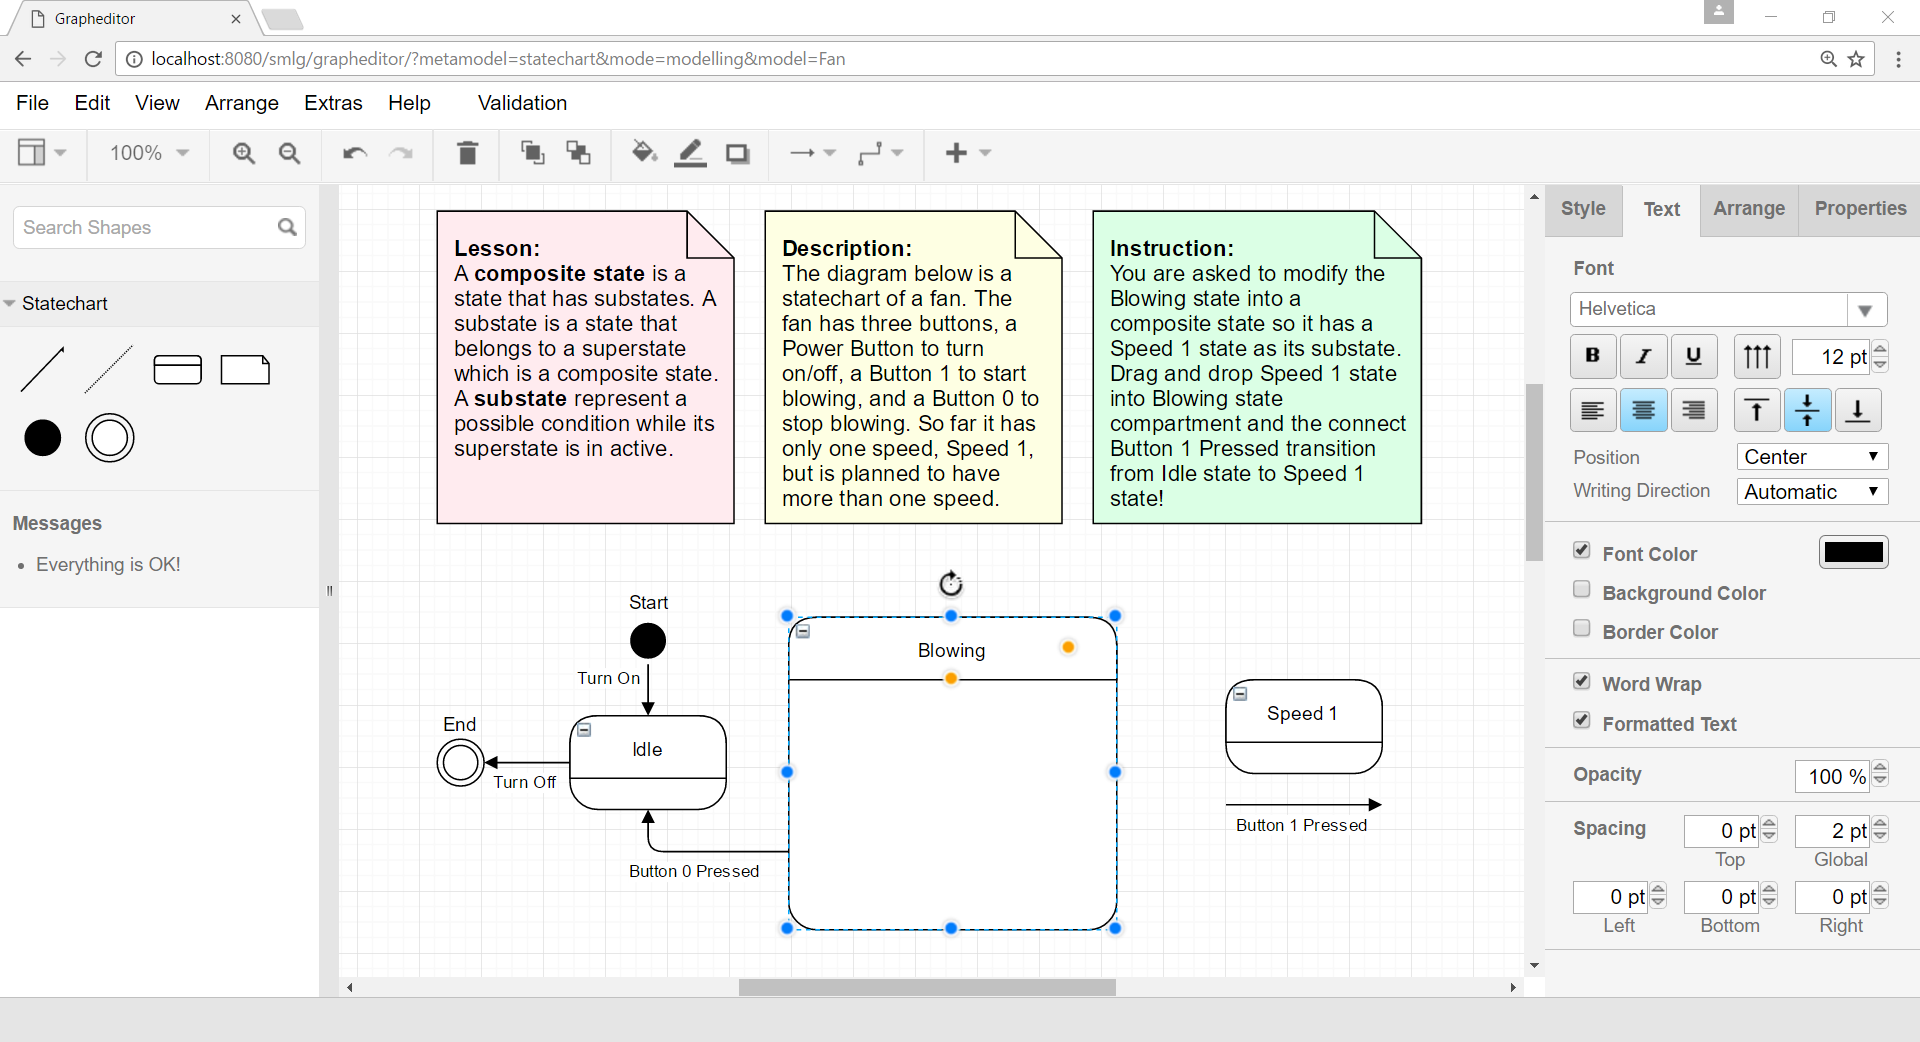
\includegraphics[width=12cm]{ide}
\caption{The MxGraph-based graphical editor to create statechart models.}
\label{ide}
\end{figure}

\begin{figure}[t!]
\centering
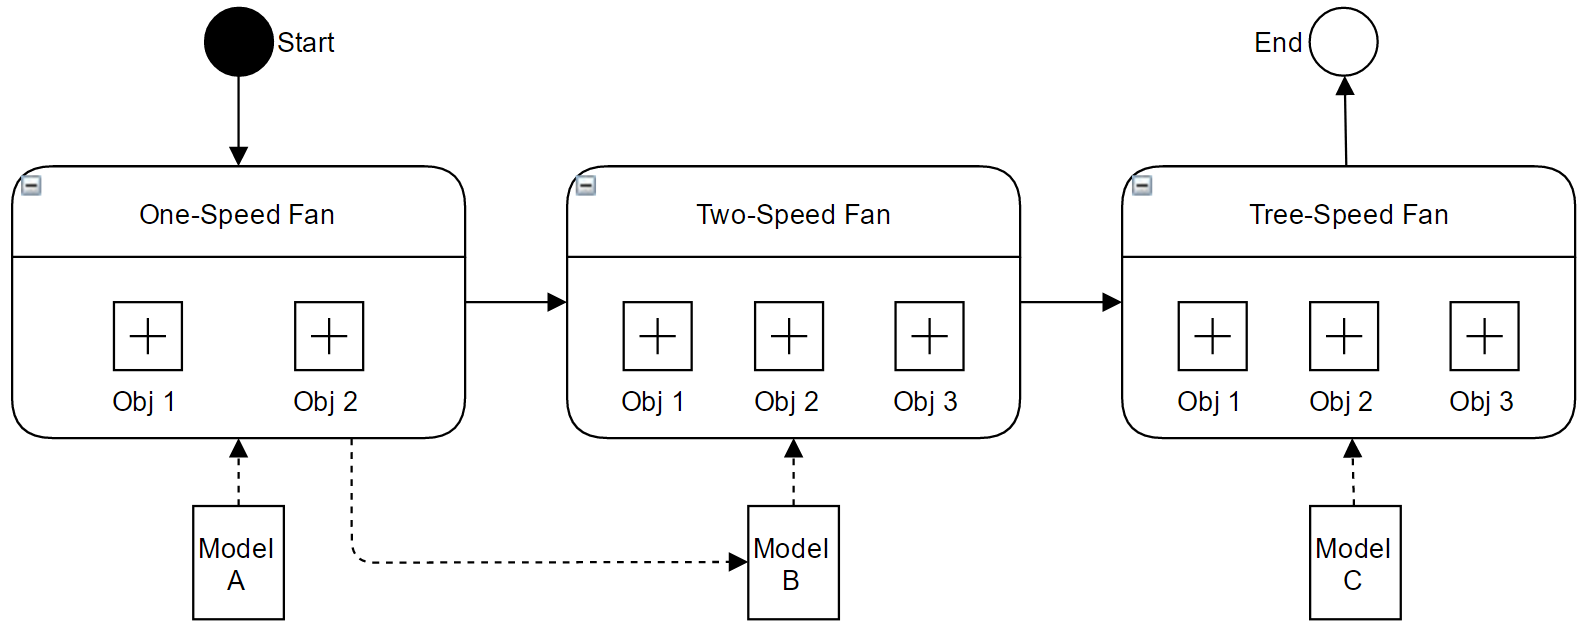
\includegraphics[width=12cm]{eoml}
\caption{A learning activity flow for learning the concept of Substates in state-machine modelling.}
\label{eoml}
\end{figure}

\begin{figure}[t!]
\centering
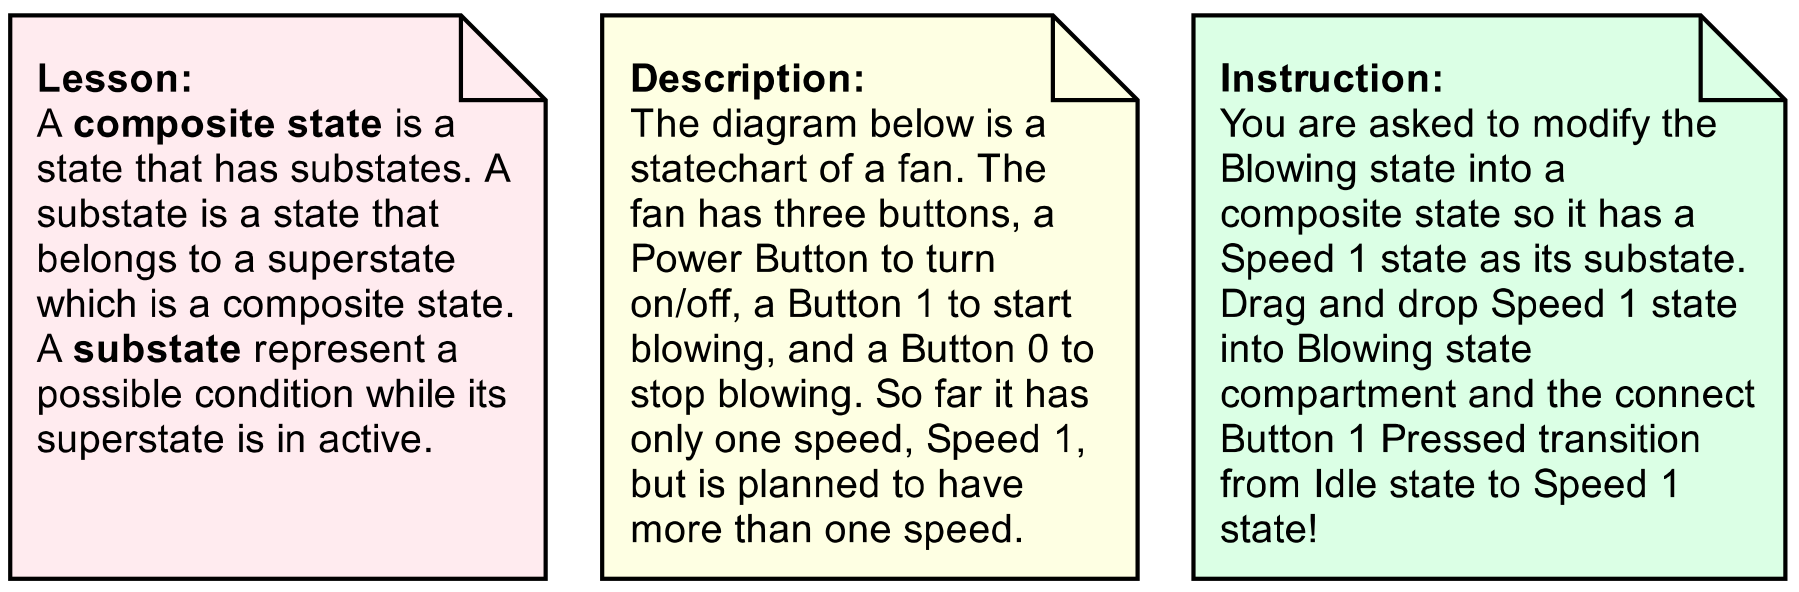
\includegraphics[width=12cm]{example-01a}
\caption{Lesson, model description, and instruction.}
\label{example-01a}
\end{figure}

\subsubsection{Create Learning Activity Model}
To teach a concept, tutors should design learning activities. In this example, a learning activity model to learn the concept of substates is created (Figure \ref{eoml}). The case is an electrical fan that has two main states, Idle and Blowing. Learners will be asked to modify the Blowing state, so it becomes a composite state with substates that represent the different speeds of blowing. The learning activity has three activities, namely One-Speed Fan, Two-Speed Fan, and Three-Speed Fan. The activities are arranged \textit{per se} to accommodate Flow state \cite{csikszentmihalyi2014toward} so learners can progress from the easiest activity to the hardest one. The activities are explained in more detail in the following subsections.
  
Each activity has a lesson and instruction properties. Lesson contains an explanation of the concepts to be taught; instruction contains commands or questions that learners need to execute or answer. Learners must meet all the objectives of an activity to move to the next activity. Each activity can consume existing models (Model A, B, and C in Figure \ref{eoml}) as its base models -- so that learners do not have to create models from scratch every time -- and produce a model (Model B in Figure \ref{eoml}) to be used in its next activity. Each model has a description property, which helps learners to understand about the model. An example of the lesson, model description, and instruction properties of the One-Speed Fan activity (Figure \ref{eoml}) is displayed in Figure \ref{example-01a}.    


\textbf{One-Speed Fan Activity}. In this activity (Figure \ref{example-01}), learners are introduced to one substate only. The activity starts with a base model, and learners are required to modify the base model (Figure \ref{example-01b}) to match the target model (Figure \ref{example-01c}). The base model corresponds to Model A in Figure \ref{eoml}, which refers to an existing base model and will be loaded once the activity is executed, so learners do not need to create the model from the start. 

The example case in this activity is a fan that has three buttons, a Power Button to turn on/off, a Button 1 to start blowing, and a Button 0 to stop blowing. So far it has only one speed, Speed 1, but is planned to have more than one speed. Learners are asked to modify the Blowing state in Figure \ref{example-01b} into a composite state by moving the Speed 1 state into the Blowing state compartment and connecting the Button 1 Pressed transition from the Idle state to the Speed 1 state. Since in Figure \ref{eoml} this activity is designed to have only two objectives, the two objectives are adjusted and defined as follow: Objective 1 ``The Blowing state contains the Speed 1 substate" and Objective 2 ``Button 1 Pressed transition connects the Idle state to the Speed 1 substate".

\begin{figure}[t!]
    \centering
    \subfloat[Base model]{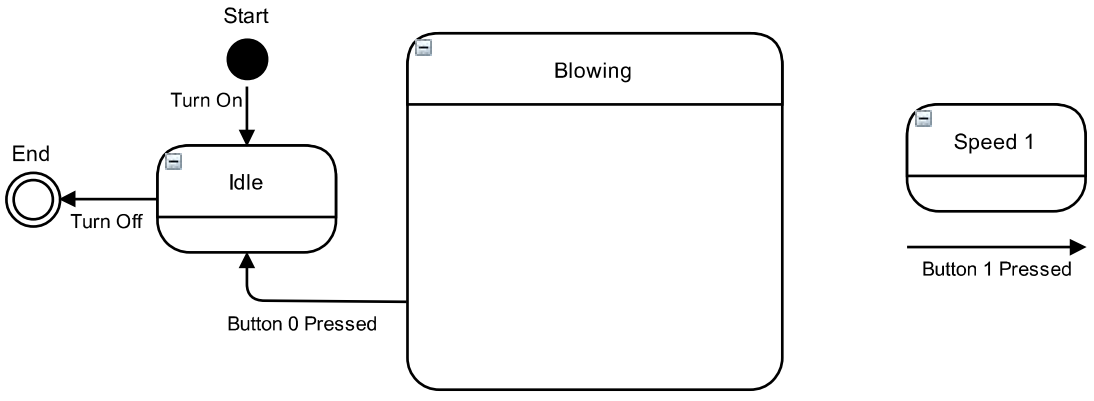
\includegraphics[width=12cm]{example-01b}	
    \label{example-01b}}
    \\
    \subfloat[Target model]{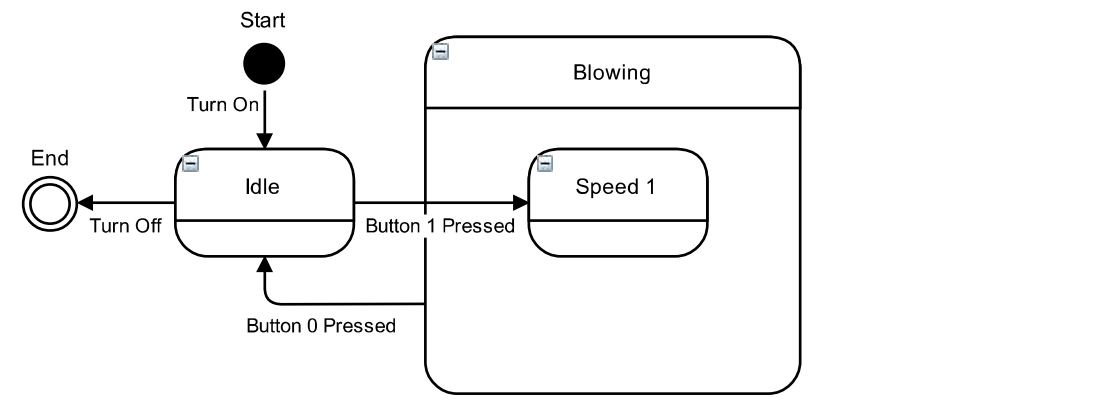
\includegraphics[width=12cm]{example-01c}
    \label{example-01c}}
	\caption{The One-Speed Fan example.}
    \label{example-01}
\end{figure}

\begin{figure}[t!]
    \centering
    \subfloat[Base model]{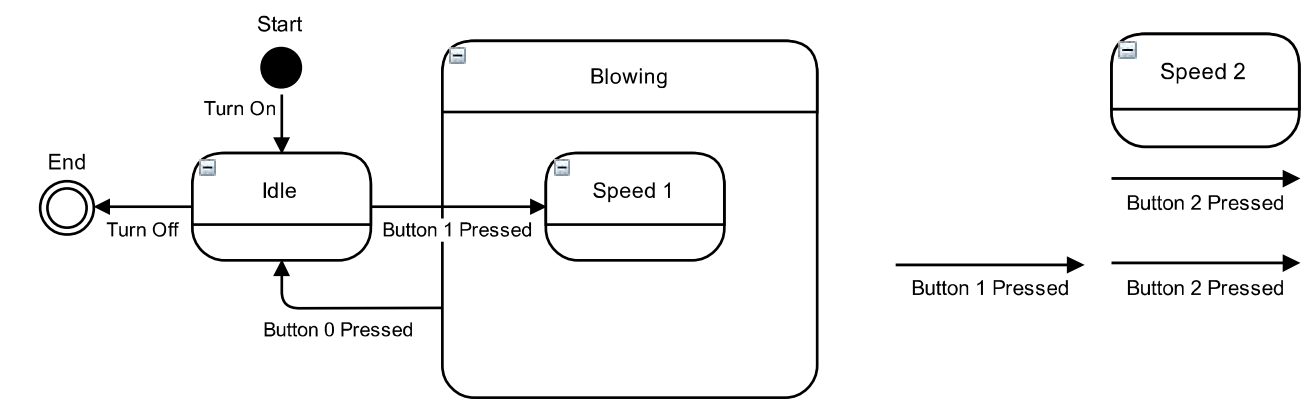
\includegraphics[width=12cm]{example-02b}	
    \label{example-02b}}
    \\
    \subfloat[Target model]{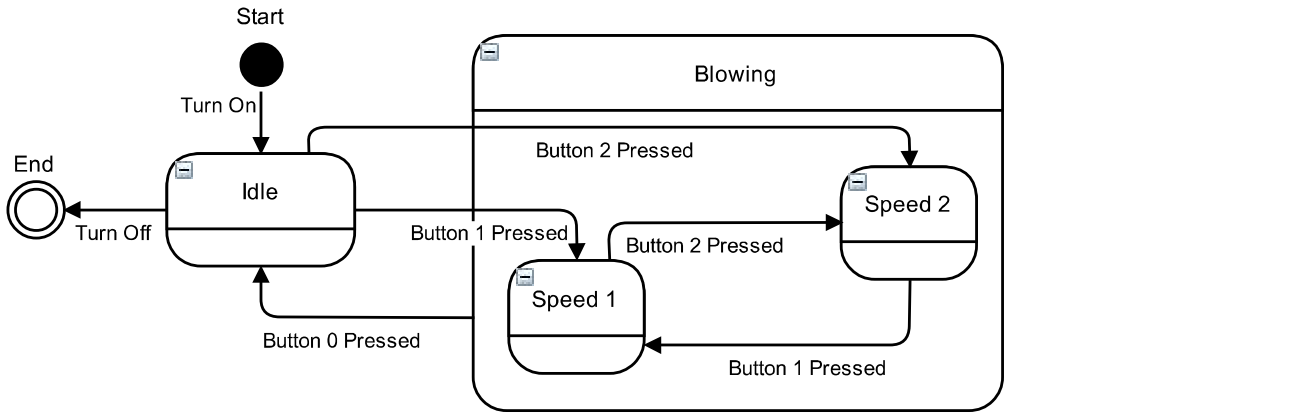
\includegraphics[width=12cm]{example-02c}
    \label{example-02c}}
	\caption{The Two-Speed Fan example.}
    \label{example-02}
\end{figure}

\begin{figure}[t!]
    \centering
    \subfloat[Base model]{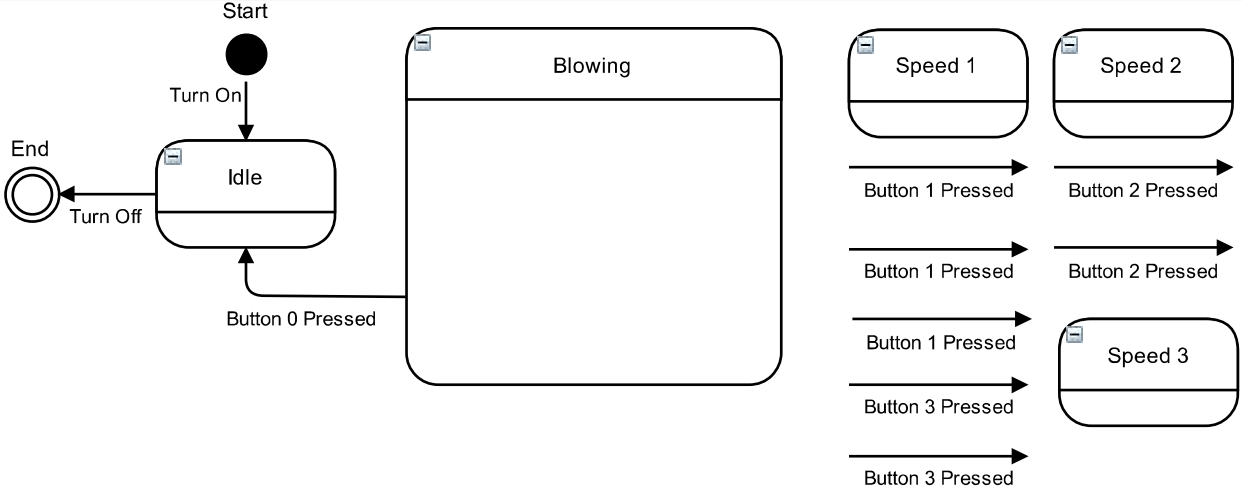
\includegraphics[width=12cm]{example-03b}	
    \label{example-03b}}
    \\
    \subfloat[Target model]{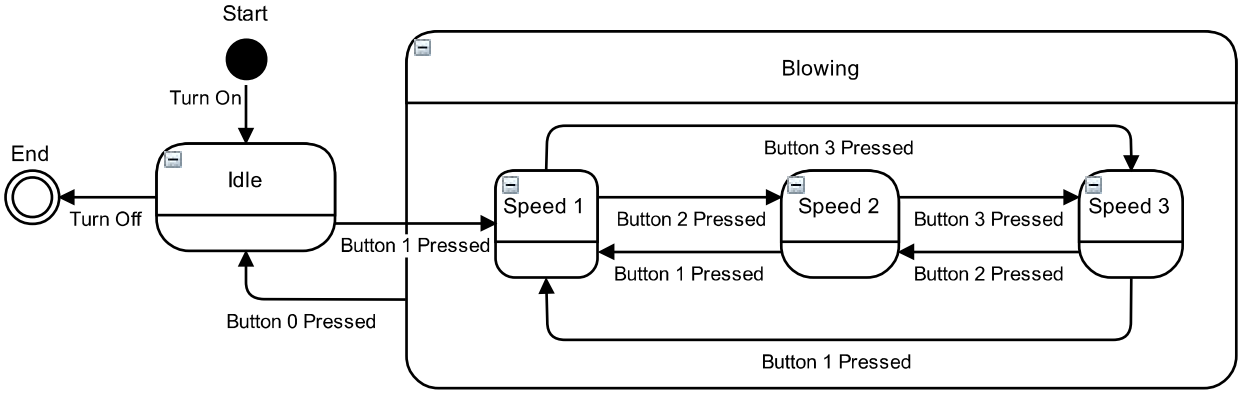
\includegraphics[width=12cm]{example-03c}
    \label{example-03c}}
	\caption{The Three-Speed Fan example.}
    \label{example-03}
\end{figure}


\begin{lstlisting}[style=interfaces,caption={Validation template for objectives in One-Speed Fan activity/level.},label=validation-template]
context Statechart {
    constraint obj_1 {
        check: self.obj_1()
        message: "FAIL: ob_1"
    }
    constraint obj_2 {
        check: self.obj_2()
        message:"FAIL: obj_2"
    }        
}
operation Statechart obj_1(): Boolean {
    return true;
}
operation Statechart obj_2(): Boolean {
    return true;
}
\end{lstlisting} 


\begin{lstlisting}[style=interfaces,caption={Validation realisation for Objective 1 in One-Speed Fan activity/level.}, label=validation-realisation]
context Statechart {
    constraint obj_1 {
        check: 
            self.obj_1()
        message:
            "FAIL: Blowing state contains Speed 1 substate"
    }
    ...
}
operation Statechart obj_1(): Boolean {
    return State.all.exists(state | state.name = "Blowing" and state.substates.exists(substate | substate.name = "Speed 1"))
}
...
\end{lstlisting} 

\textbf{Two-Speed Fan Activity}. The Two-Speed Fan activity (Figure \ref{example-02}) consumes the model that has been produced in the first activity (Model B in Figure \ref{eoml}). Any model generated in the previous activity becomes the base model for modelling in this activity. In accordance with the Flow concept \cite{csikszentmihalyi2014toward}, this second activity should be more challenging. Therefore, the activity (Figure \ref{example-02}) challenges learners with one additional state and three new transitions. Now the case has changed. The fan has an extra button, Button 2, to support 2-speed blowing. When Button 1 is pressed, the fan blows in speed 1 and when Button 2 is pressed, the fan blows in speed 2. Thus, learners need to modify the Blowing state into a composite state, so that it has two-speed states. The fan can move from the Idle state to the Speed 1 state, from the Idle state to the Speed 2 state, and from the Speed 1 state to the Speed 2 state or \textit{vice versa}.

\textbf{Three-Speed Fan Activity}. The Three-Speed Fan activity (Figure \ref{example-03}) should be harder than the second activity. The fan now supports 3 speeds of blowing, but it has been modified so it cannot go directly to Speed 2 or Speed 3 without firstly going to a state with a lower speed. In other words, the transition from Idle can only go to Speed 1 for the fan to start blowing. Thus, starting from the model C as the base model (Figure \ref{eoml}), learners are required to modify the Blowing state into a composite state with 3 speeds of blowing and to only allow a transition from Idle to Speed 1.

\subsubsection{Generate Game}
After constructing the learning activity (Figure \ref{eoml}), designers can now generate a path of levels (or stages). Each generated level corresponds to an activity defined in the learning activity and has an EVL template for validation. The EVL template is shown in Listing \ref{validation-template} which can be extended by designers to write constraints that fit the level scenarios and objectives. The number of constraints and operations in the template corresponds to the number of objectives defined in the level's learning activity activity in Figure \ref{eoml}. As an example, implementation of validation, Listing \ref{validation-realisation} shows the EVL code to check whether the Blowing state has a Speed 1 substate, as intended by Objective 1 in One-Speed activity.   


\subsubsection{Play Game}
After generating the learning activity into a path of ordered levels and defining its levels' validation, learners can choose the path and play its levels as depicted in Figure \ref{path}. When learners choose the first level, an MxGraph-based editor is displayed, and the lesson, model description, instruction, objectives, and base model are presented to learners. Learners can then start to modify the base model to reach the target model. 

\begin{figure}[t!]
\centering
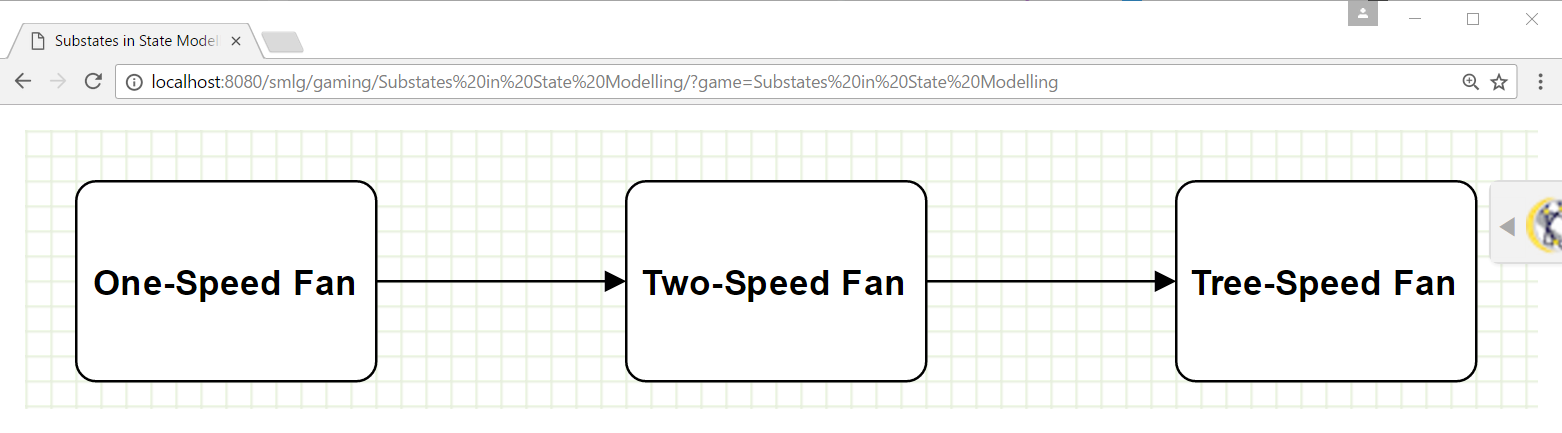
\includegraphics[width=12cm]{path}
\caption{The path for learning substate concept with its levels.}
\label{path}
\end{figure}    

Every attempt to change the model triggers an operation to validate the current model using the defined EVL constraints to assess whether the model has met the current level's objectives. If not, feedback is displayed to learners indicating the objectives that have not been satisfied. For example, in Figure \ref{example-fail-messages}, the Speed 1 substate has not been put into the Blowing state even though the Button 1 Pressed transition has connected the Idle state to the Speed 1 substate. If all objectives have been fulfilled, the level is considered completed, an appropriate message is produced to provide positive reinforcement, and the learner can proceed to the next level.  

\begin{figure}[t!]
\centering
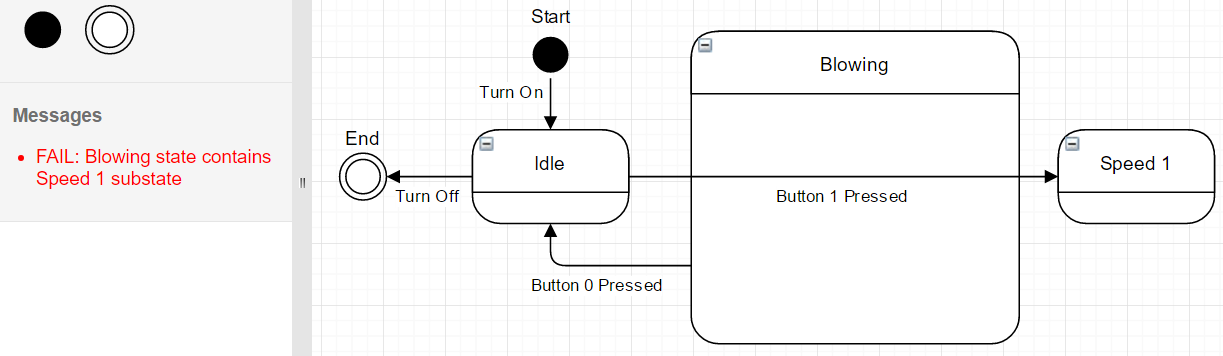
\includegraphics[width=12cm]{example-fail-messages}
\caption{A message is displayed to learners indicating the objective that has not been fulfilled.}
\label{example-fail-messages}
\end{figure}  

\subsection{Evaluation Plan}
\label{Evaluation Plan}
Two forms of assessment have been planned to evaluate the framework. The first assessment is to measure the effectiveness of modelling games vs. class-based lecturing using controlled experiments involving undergraduate and postgraduate students. Subjects will be grouped into two groups, an experimental group, and a control group. While the control group will only learn from attending class-based lecturing, the other group will also learn using games. Both will be tested with relevant problems before and after teaching to measure their improvement. The gap between the two group will be used to measure the effect of the games. Even though this evaluation is feasible since an adequate number of software engineering students are available, challenges still exist. The quality of the class-based lecturing, the problems given in the tests, and the games should be consistent, ensuring that they carefully designed to address the same educational objectives. The other challenge is to have the two groups of subjects have balanced quality and distribution. 
  
The second assessment is to measure the development effort needed to develop a complete game for a non-trivial modelling language, and the savings realised using the model-driven approach. The assessment will be tested on developers that have considerable background in developing games, which also implies a challenge since it is hard to get developers that have such qualification and are willingly participate as subjects. The measures will be on time used to complete the game and ratio between lines of code written and lines of code generated. Subjective feedback from the developers will also be useful to describe the quality of the framework. 

\section{Communication}
The progress of this research should be communicated to a larger audience. So far, only two papers have been made for publication. The first paper has been published in a doctoral symposium setting, and the other one is already submitted to a conference and waiting for review. The detail of the publication can be found in the Publications section (Chapter \ref{Publications}).

\chapter{Research Plan}
\label{Research Plan}
This year, 2017, time will be spending much on developing a prototype, with an experiment and survey will be conducted in between October and December in the UK. The experiment and survey are to execute the evaluation plan in Subsection \ref{Evaluation Plan}. The same experiment and survey will also be conducted in 2018 but are planned to be executed in Indonesia. The year 2019 will be used mostly for thesis writing. The research timetable is displayed in Table \ref{Research Timetable}. 

\begin {table}[th]
\caption {Research Timetable} 
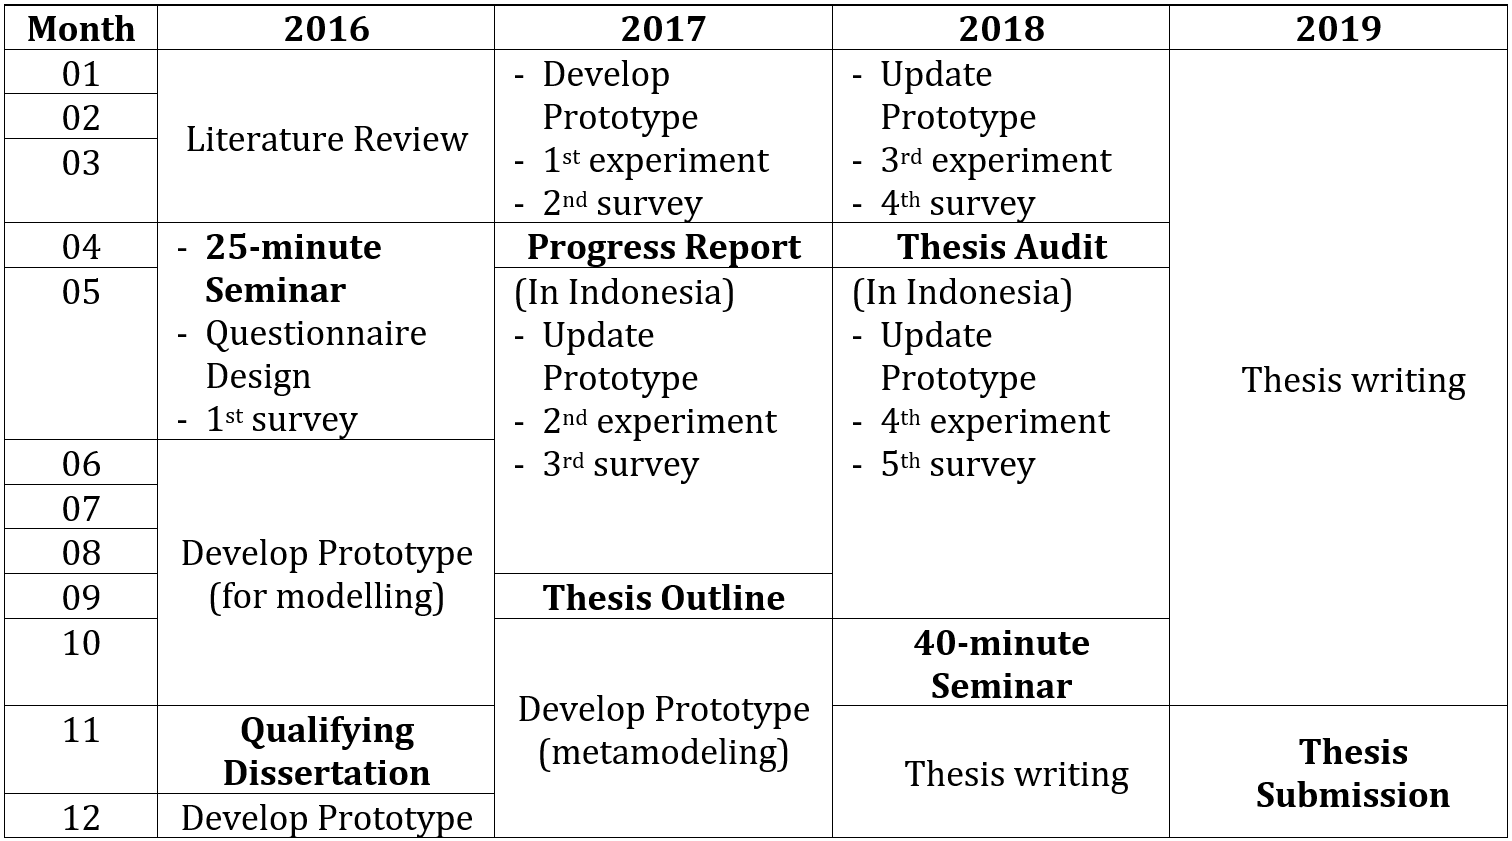
\includegraphics[width=\textwidth]{timetable}
\label{Research Timetable}
\end{table}

The next work is completing the prototype development, such as adding multiple-choice gameplay, semantic equivalence validation, and reward mechanisms. Two facilities will also be added: a fine-grained logging framework that will allow game designers to replay solutions and understand how users interact with the game and a facility that monitors the progress of learners. 


\chapter{Publications}
\label{Publications}
Papers have been published in the following conferences or journals: 
\begin{enumerate}
 \item A. Yohannis, ``Gamification of software modelling learning,'' in
 \textit{the ACM/IEEE 19th International Conference on Model Driven Engineering Languages and Systems (MODELS 2016) Doctoral Symposium}. CEUR, 2016. \cite{Yohannis2016}.
 \item A. Yohannis, D. Kolovos, and F. Polack, ``Towards Model-Driven Gamified Software Modelling Learning,'' in \textit{the ACM/IEEE 20th International Conference on Model Driven Engineering Languages and Systems (MODELS 2017)}. (submitted, in review).
\end{enumerate}

\bibliographystyle{IEEEtran}
\bibliography{references}




%\begin{appendices}
%\end{appendices}

\end{document}






